\documentclass[11pt]{article}
\usepackage[a4paper, margin=20mm]{geometry}
 

\usepackage{amsmath}
\usepackage{physics}

\usepackage{graphicx}
\graphicspath{ {./figs/} }
\usepackage{subfig}

%\renewcommand{\baselinestretch}{2}
\usepackage{setspace}
\doublespacing
\usepackage{titlesec}
\usepackage{authblk}
\usepackage{titling}

% \usepackage[backend=bibtex,style=authoryear,natbib=true]{biblatex} % Use the bibtex backend with the authoryear citation style (which resembles APA)
\usepackage[backend=biber,
style=authoryear,
citestyle=apa]{biblatex}
\addbibresource{Reference.bib} % The filename of the bibliography
% \usepackage[autostyle=true]{csquotes} % Required to generate language-dependent quotes in the bibliography
\usepackage{enumitem}
% \makeatletter
% \newcommand{\setword}[2]{%
%   \phantomsection
%   #1\def\@currentlabel{\unexpanded{#1}}\label{#2}%
% }
% \newcommand{\citebracks}[2][]{
%    \citeauthor{#2} (\citeyear[#1]{#2})
% }

% \makeatother
% \usepackage{floatrow}

\setlength{\droptitle}{-9em}   % This is your set screw


\titlespacing\section{0pt}{0pt plus 0pt minus 0pt}{0pt plus 2pt minus 2pt}
\titlespacing\subsection{0pt}{0pt plus 4pt minus 2pt}{0pt plus 2pt minus 2pt}
\titlespacing\subsubsection{0pt}{0pt plus 4pt minus 2pt}{0pt plus 2pt minus 2pt}


\title{The Future of Work - 12653}
\author{Author: Nian Yang Terence Tan \and Supervisor: Dr. Michael A Osborne}

\begin{document}

\maketitle


\section{Overview of the project}
The world population is ageing over the next few decades (\cite{science}). The rising elderly to working age population ratio is increasing and will continue to do so (\cite{WHO}). This trend is known as an ageing population, and will strain the public and social services of many countries around the world (\cite{publicservicesstrain}). As one of the key social challenges facing the world for the next few decades, it would be interesting to examine how an ageing population will affect the economy, and in particular, the job market.

\section{Key project objectives}
In this project, we aim to examine the relationship between the age distribution within occupations and the degree of automation (both present and future) of those occupations. We might also look into any correlations with the skills/knowledge required for those occupations. This will all be done using a Bayesian non-parametric machine learning technique called Gaussian Process (\cite{GaussianProcess}).

The original goal was to extrapolate the changes in distribution of age groups within occupations over the next few years, but this was deemed unfeasible due to the limited amount of time-series data.

% \begin{figure}[!htb]
%     \centering
%     \subfloat[Without White Kernel (RMS error = 1.748)]{\includegraphics[width=8cm]{Figures/Graph 1.png}\label{fig:fig1}}
%       \hfill
%     \subfloat[With White Kernel (RMS error = 0.667)]{\includegraphics[width=8cm]{Figures/Graph 2.png}\label{fig:fig2}}
%     \hfill
%     \caption{Predicted values}
%   \end{figure}
  
\section{Progress to date}
Over the summer, I have looked into Gaussian Processes and completed an online laboratory assignment designed by my supervisor. I hae also read past papers looking into similar areas of research.

Potential data sources have already been identified. The distribution of age groups within occupations are published by the US Bureau of Labour Statistics (BLS)\footnote{https://www.bls.gov}, and go back to 2011. We can find the skills and knowledge associated with the various occupations on O*NET Online\footnote{https://www.onetonline.org}.

A GitHub repository for this project has also been created\footnote{https://github.com/terencetan-c/4YP-The-Future-of-Work}; it contains codes, reports, etc.


  

    
  \section{Immediate tasks}
  Data wrangling work has already been started on the BLS data in order to standardise the data sets across the years. The differences are mainly due to changes to the Standard Occupational Classification (SOC) system. The SOC codes would allow us to map between the the BLS and the O*NET dataset. Since the changes to the SOC codes are quite complex, it was deemed unrealistic to automate the data wrangling. Instead, it would be done manually, which would still be manageable given that only about a hundred rows of data have been flagged for closer inspection. All the details of the data wrangling process can be found in an excel file on the GitHub repository.

  \section{Plan of work to the end of the project}
  Once the data wrangling is completed, figures and graphs will be produced from the standardised BLS data to give us a clearer picture of the data. We will then move on to selecting an appropriate Gaussian Process and train our model on the BLS data. If things go well, we may then look at the O*NET data and incorporate it into this project. While doing all of these, I will start working on the report and the presentation.

  A high-level Gantt Chart was created to allow us to track our progress over time; the list view of the chart can be seen in Figure \ref{fig:gantt}.

  \begin{figure}[!htb]
    \centering
    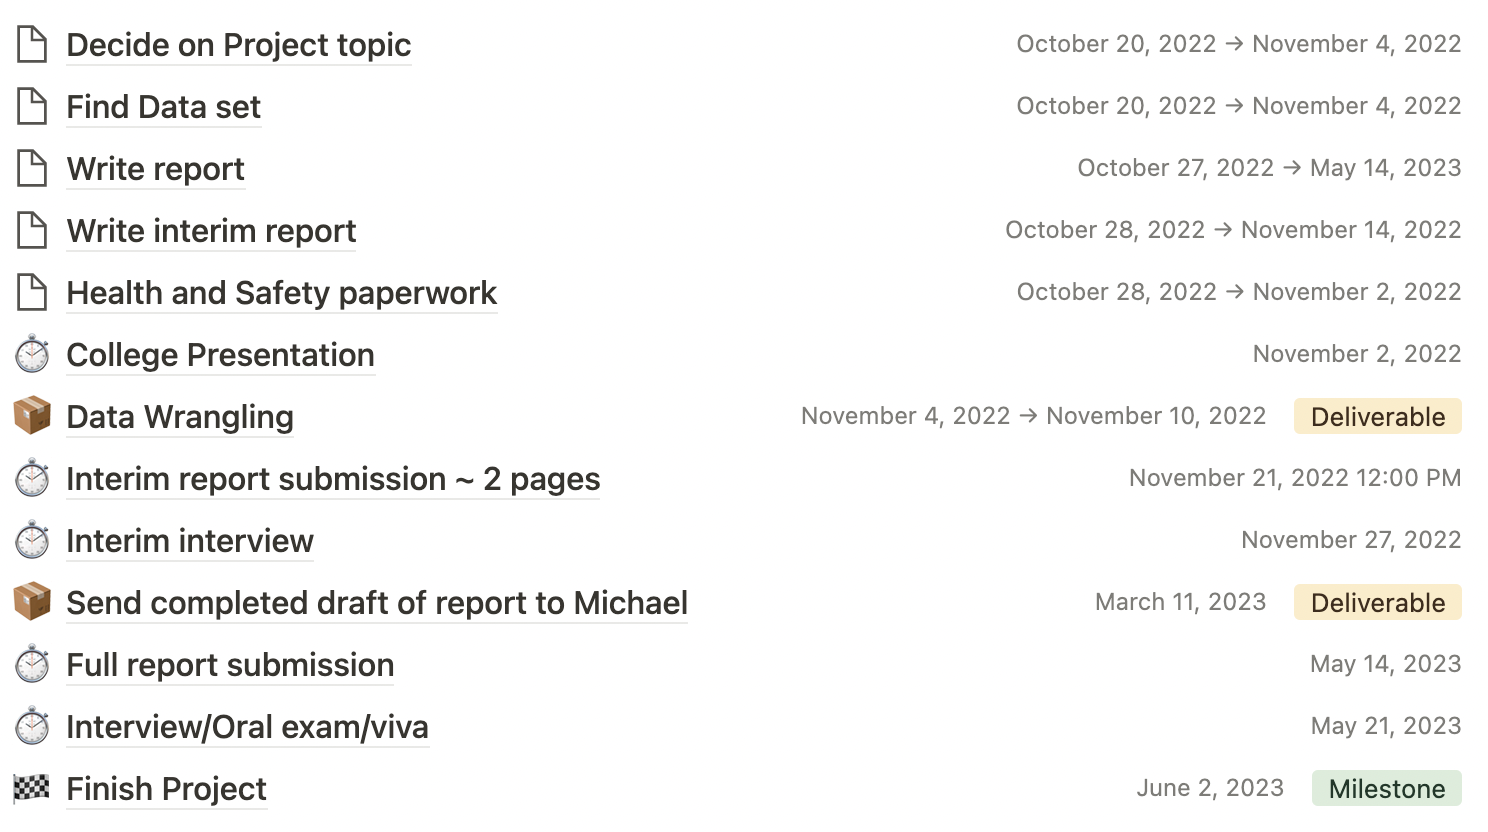
\includegraphics[width=12.5cm]{/Users/terencetan/Documents/Uni stuff/Engineering Science/4YP/4YP-The-Future-of-Work/Report/Figures/Gantt List.png}
    \caption{Gantt Chart in List View}
    \label{fig:gantt}

  \end{figure}

    % \setstretch{1.4}
    \printbibliography[heading=bibintoc]

\end{document}
